\section{Results}\label{sec:results}

\subsection{Logical error rates}

Table~\ref{tab:ler} lists the logical errors of PyMatching alone and of the pre-decoder followed by PyMatching on the
same shots, for both networks, both noise levels and both arithmetics, together with the improvement factors NVIDIA
published for the X basis \cite{chamberland2026predecoder}; Fig.~\ref{fig:ler} compares the X basis factors.

\begin{table}[t]
\caption{Logical errors over both bases (X and Z, each with the stated number of shots) of PyMatching alone and of
the pre-decoder followed by PyMatching on the same shots, with $T=d$ rounds. Ratio, X: improvement factor in the X
basis (PyMatching errors divided by errors with the pre-decoder); NVIDIA, X: the published factor for the same
network, $p$ and $d$ (Tables 4 and 5 of \cite{chamberland2026predecoder}).}\label{tab:ler}
\centering
% generated by scripts/make_numbers.py
\begin{tabular}{@{}llrrrrrrr@{}}
\toprule
Network & Arithmetic & $d$ & $p$ & Shots per basis & PyMatching & With pre-decoder & Ratio, X & NVIDIA, X \\
\midrule
Fast & FP32 & 9 & 0.003 & 1{,}048{,}576 & 2{,}605 & 2{,}479 & 1.08 & 1.10 \\
Fast & INT8 & 9 & 0.003 & 65{,}536 & 154 & 154 & 0.80 & 1.10 \\
Fast & FP32 & 13 & 0.003 & 1{,}048{,}576 & 519 & 586 & 0.90 & 0.91 \\
Fast & FP32 & 9 & 0.006 & 1{,}048{,}576 & 61{,}392 & 51{,}883 & 1.17 & 1.24 \\
Fast & INT8 & 9 & 0.006 & 65{,}536 & 3{,}887 & 3{,}317 & 1.14 & 1.24 \\
Accurate & FP32 & 13 & 0.003 & 524{,}288 & 223 & 176 & 1.29 & 1.32 \\
Accurate & FP32 & 13 & 0.006 & 262{,}144 & 11{,}577 & 6{,}747 & 1.72 & 1.76 \\
Accurate & INT8 & 13 & 0.006 & 65{,}536 & 2{,}849 & 1{,}922 & 1.51 & 1.76 \\
\botrule
\end{tabular}

\end{table}

\begin{figure}[t]
\centering
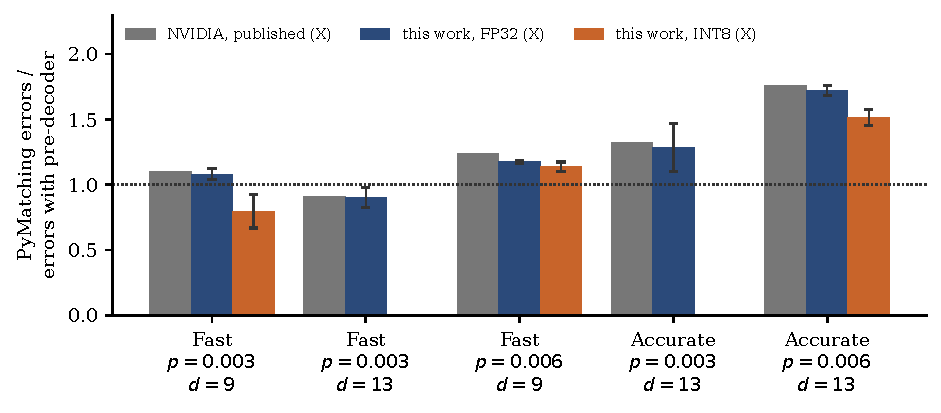
\includegraphics[width=\textwidth]{figures/fig_ler.pdf}
\caption{Improvement factor of the pre-decoder over PyMatching alone in the X basis: NVIDIA's published values and
the values measured here with NVIDIA's evaluation code, for the floating point (FP32) and the integer (INT8)
networks. Error bars: one standard deviation from the counts of logical errors. Values below the dotted line mean
that the pre-decoder increases the logical error rate.}\label{fig:ler}
\end{figure}

\textbf{Agreement with the published values.} With NVIDIA's own evaluation code our measurements follow the published
factors in the X basis. The Fast network at $p=0.003$ gives \NumRatioXFastFpNineLow{} at $d=9$ and
\NumRatioXFastFpThirteenLow{} at $d=13$ (\NumShotsFastFpThirteenLow{} shots per basis each), against 1.10 and 0.91
published, and at $p=0.006$, $d=9$ \NumRatioXFastFpNineHigh{} (\NumShotsFastFpNineHigh{} shots per basis), against
1.24. The Accurate network at $d=13$ gives \NumRatioXAccFpThirteenLow{} at $p=0.003$ (\NumShotsAccFpThirteenLow{} shots
per basis) and \NumRatioXAccFpThirteenHigh{} at $p=0.006$ (\NumShotsAccFpThirteenHigh{} shots per basis), against 1.32
and 1.76. Every factor we measure is within 0.07 of the published one and slightly below it.

\textbf{When the pre-decoder pays off.} The small Fast network gives at best a modest gain: at $p=0.003$ it lowers the
logical error rate by a factor of only \NumRatioFastFpNineLow{} over both bases at $d=9$ and raises it at $d=13$
(\NumRatioFastFpThirteenLow{}), in agreement with the factor below one that NVIDIA reports for this network at this
noise level. The Accurate network, with two more layers and a receptive field
of 13, lowers the logical error rate by a factor of \NumRatioAccFpThirteenHigh{} over both bases at $p=0.006$ and by
\NumRatioAccFpThirteenLow{} at $p=0.003$, both at $d=13$. The gains quoted for the network family therefore depend on
the network size and the noise level, and a hardware implementation should target the larger network.

\textbf{Integer arithmetic.} The integer model of the Fast network gives a factor of \NumRatioFastIntNineHigh{} over
both bases at $p=0.006$, $d=9$ (\NumShotsFastIntNineHigh{} shots per basis), against \NumRatioFastFpNineHigh{} in
floating point, and the integer Accurate network gives \NumRatioAccIntThirteenHigh{} at $p=0.006$, $d=13$
(\NumShotsAccIntThirteenHigh{} shots per basis), against \NumRatioAccFpThirteenHigh{}. The integer model thus keeps
the gain of the four layer network but loses about a third of the gain of the six layer network, plausibly because the rounding of
the activations accumulates over five hidden layers; with \NumIntAccAfter{} errors against \NumIntAccExpected{}
expected on the same shots from the floating point factor, the loss is well outside the counting uncertainty. At $p=0.003$, $d=9$ the integer Fast network gives
\NumRatioFastIntNineLow{} over both bases, with too few errors (\NumShotsFastIntNineLow{} shots per basis) to
distinguish it from the floating point network. Since the kernel output is bit exact with the integer model
(Section~\ref{sec:hw}), these are the logical error rates the cards deliver.

\subsection{Hardware}\label{sec:hw}

\textbf{Implementation.} After routing and post route physical optimization, the two instance design misses the
300~MHz target by a worst negative slack of \NumWns{}~ns, and Vitis lowers the kernel clock to \NumKernelMhz{}~MHz. Table~\ref{tab:resources} lists the routed resources of one
instance. The routed design uses more DSP blocks and BRAM and fewer URAM blocks than the HLS estimate, because the
implementation maps part of the products to DSP blocks and part of the on chip memories to BRAM; DSP blocks are the
largest share, at less than half of one SLR.

\begin{table}[t]
\caption{Routed resources of one kernel instance (the second instance is within 2\% of these values), as reported
by Vivado after implementation, and their share of one SLR of the U55C.}\label{tab:resources}
\centering
% generated by scripts/make_numbers.py
\begin{tabular}{@{}lrr@{}}
\toprule
Resource & One instance & Percent of one SLR \\
\midrule
LUT & 38{,}496 & 8.9 \\
Flip flops & 50{,}553 & 5.8 \\
DSP blocks & 1{,}296 & 43.1 \\
BRAM (36 kbit) & 269 & 40.0 \\
URAM & 114 & 35.6 \\
\botrule
\end{tabular}

\end{table}

\textbf{Bit exactness.} All \NumCheckCount{} checks (two networks on four cards) passed: the output bits of all \NumCheckInstances{} instance runs equal those of the integer model for every site
and output channel of the test windows. Since the kernel computes the integer model exactly for any calibration, the logical error rates of the integer
model in Table~\ref{tab:ler} are those of the cards.

\textbf{Throughput.} Table~\ref{tab:throughput} and Fig.~\ref{fig:throughput} give the measured throughput. One card
processes \NumOneFast{} windows per second of the Fast network at $d=9$ and \NumOneAcc{} of the Accurate network at
$d=13$, and four cards \NumFourFast{} and \NumFourAcc{}: the scaling from one to four cards is \NumScaleFast{} and
\NumScaleAcc{}, as expected for nodes that exchange no data, and the three repetitions of each point agree to within
one window per second. One instance reaches \NumModelEffFast{}\% (Fast) and \NumModelEffAcc{}\% (Accurate) of the
throughput predicted by the cycle model at \NumKernelMhz{}~MHz, so the transfers of the windows and of the output bits
are hidden behind the computation and the kernel runs at the rate its schedule allows. In products per second, four
cards perform \NumTmacFast{}$\times10^{12}$ (Fast) and \NumTmacAcc{}$\times10^{12}$ (Accurate) useful 8 bit
multiply accumulate operations per second. During the measurements the card temperatures stayed at or below
\NumTempMax{}~$^\circ$C.

\begin{table}[t]
\caption{Throughput in windows per second on one, two and four cards (two instances per card), median and range of
three repetitions of about 20 seconds each. Scaling: throughput divided by the number of cards times the throughput of
one card.}\label{tab:throughput}
\centering
% generated by scripts/make_numbers.py
\begin{tabular}{@{}lrrrrr@{}}
\toprule
Network & Cards & Windows/s (median) & Range & Per card & Scaling \\
\midrule
Fast, $d=9$ & 1 & 623 & 622 to 623 & 623 & 1.00 \\
Fast, $d=9$ & 2 & 1{,}245 & 1{,}245 to 1{,}245 & 622 & 1.00 \\
Fast, $d=9$ & 4 & 2{,}490 & 2{,}490 to 2{,}490 & 622 & 1.00 \\
\midrule
Accurate, $d=13$ & 1 & 127 & 127 to 127 & 127 & 1.00 \\
Accurate, $d=13$ & 2 & 255 & 255 to 255 & 127 & 1.00 \\
Accurate, $d=13$ & 4 & 509 & 509 to 509 & 127 & 1.00 \\
\botrule
\end{tabular}

\end{table}

\begin{figure}[t]
\centering
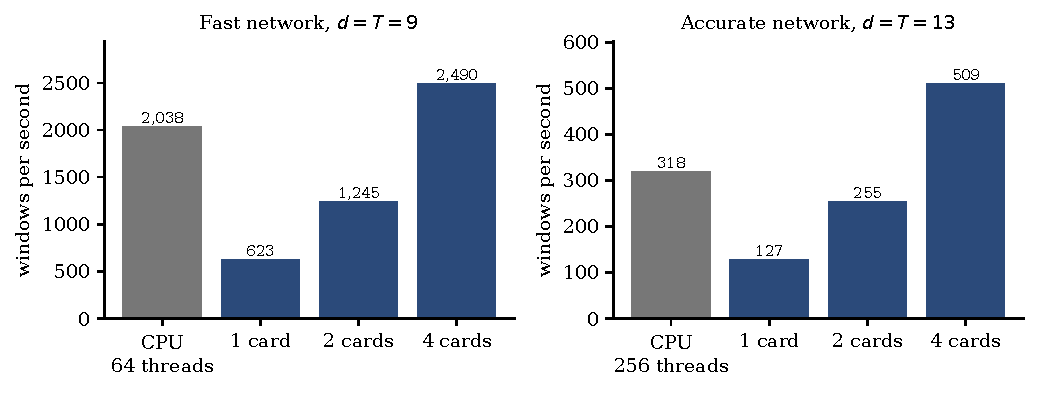
\includegraphics[width=\textwidth]{figures/fig_throughput.pdf}
\caption{Throughput of the floating point networks in PyTorch on the host CPU (best thread count and batch size) and of
the integer networks on one, two and four cards.}\label{fig:throughput}
\end{figure}

\textbf{Comparison with the host CPU.} PyTorch on the host reaches at best \NumCpuFastBest{} windows per second for
the Fast network (\NumCpuFastBestThreads{} threads, batch size \NumCpuFastBestBatch{}) and \NumCpuAccurateBest{} for
the Accurate network (\NumCpuAccurateBestThreads{} threads, batch size \NumCpuAccurateBestBatch{}); at batch size one
it reaches \NumCpuFastOne{} and \NumCpuAccurateOne{}, that is \NumCpuFastOneMs{}~ms and \NumCpuAccurateOneMs{}~ms per
window. Four cards are therefore only \NumSpeedFast{} times (Fast) and \NumSpeedAcc{} times (Accurate) faster than the
host CPU at its best setting, and one card is slower than the host. The throughput of the CPU varies between the two
repetitions of a point, by a median of \NumCpuVarMedFast{}\% (Fast) and \NumCpuVarMedAccurate{}\% (Accurate) and by up
to \NumCpuVarMaxAccurate{}\% at single points; the comparison uses the best repetition, which favours the CPU.

\textbf{Latency.} With one window per launch and one launch in flight, a window takes \NumLatFast{}~ms (Fast, $d=9$)
and \NumLatAcc{}~ms (Accurate, $d=13$) from the start of the transfer to the card until its bits are back on the host.
The computation alone takes \NumComputeMsFast{}~ms and \NumComputeMsAcc{}~ms according to the cycle model; the
remaining \NumLatOverheadFast{}~ms and \NumLatOverheadAcc{}~ms cover the transfers, the kernel launch through XRT and
the loading of the weights from HBM, which each launch repeats.
